\section{Jets} \label{sec:objects:jets}

The LHC produces a massive ammount of QCD radiation as a result of the large
cross section for jets and dijets from $pp$ collisions (see
\Cref{fig:xsection_measurements}).  However, reconstructing these objects into
the quark or gluon object that created the jet proves to be quite challenging
due to the stochastic nature of the hadronization process discussed in
\Cref{sec:theory:qcd}.  This issue is further complicated by the large number
of underlying events due to pile-up discussed in \Cref{sec:lhc:pileup}, meaning
that multiple jets may be very close to each other or even overlapping.  So
instead of quark or gluon objects we instead cluster energy deposits and
combine them with associated charged tracks to create jet objects which can
originate from either a gluon or quark.  This also makes sense from a
theoretical standpoint as colored objects can never be directly observed, but
the colorless neutral and charged hadrons they hadronize into are easiy
observed.

Jet clustering algorithms are used to create these collections of tracks and
energy deposits, known as "jets".  The most common clustering algorithm are the
$k_{t}$, Cambridge-Aachen, and anti-$k_{t}$ algorithms \cite{Cacciari:2008gp}.
These algorithms work by iteratively applying the following rules to the
collection of momentum deposition objects:

\begin{enumerate}
  \item Define the distance $d_{iB}$ between the object $i$ and the beamline $B$ in terms of the transverse momentum $p_{T}$ and $P$ which determines the effect of the energy in the clustering algorithm: \[ d_{iB} = p_{Ti}^{2P} \]
  \item Compute the pairwise distance $d_{ij}$ between objects $i$ and $j$: \[ d_{ij} = \textrm{min}\left(p_{Ti}^{2P}, p_{Tj}^{2P}\right) \frac{\DeltaR_{ij}^{2}}{R^{2}} \] where $\DeltaR_{ij}^{2} = \left(\eta_{i} - \eta_{j}\right)^{2} + \left(\phi_{i} - \phi_{j}\right)^{2}$ is the geometric term dependent on rapidity $\eta$ and the azimuthal angle $\phi$.  $R$ is a parameter which controls the size of the jet.
  \item Choose the smallest distance $d_{\text{min}}$ out of the list of distances you've just created: \[ d_{\mathrm{min}} \in \left\{\left\{d_{ij}\right\},\left\{d_{iB}\right\}\right\} \] 
  \item If $d_{\text{min}}$ is the distance between an object, $i$, and the beamline: \[ d_{\mathrm{min}} \in \left\{d_{iB}\right\} \] label this object a jet and remove it from the list
  \item If $d_{\text{min}}$ is the distance between some objects $i$ and $j$: \[ d_{\mathrm{min}} \in \left\{d_{ij}\right\} \] merge objects $i$ and $j$ into a new object $k$, add $k$ to the object collection and remove objects $i$ and $j$.
  \item Repeat until all objects have been clustered into jets and the object collection is empty
\end{enumerate}

In the above iterative process the choice of parameter P corresponds to three choices of jet clustering algorithm:

\begin{enumerate}

  \item[$P = 1$] This defines the $k_{t}$ algorithm \cite{Catani:1993hr}.  Here the algorithm prioritizes the clustering of soft objects first and then gradually moves on to harder objects.  This has the effect of creating irregular shaped jets that evolve from the "outside-in" as seen in \Cref{sec:objects:kt}
  \item[$P = 0$] This defines the Cambridge-Aachen algorithm \cite{Dokshitzer:1997in}.  In this case the effect of the energy of the jet is ignored and instead the jets are clustered entirely based off of their geometric distance.  Again this results in irregular shaped jets as seen in \Cref{sec:objects:Cam_Aachen}
  \item[$P = -1$] This defines the anti-$k_{t}$ algorithm \cite{Cacciari:2008gp}.  This algorithm prioritizes the clustering of hard objects first and then clusters the surrounding softer objects.  This results in mostly cone like jets which center on the hardest object(s) as seen in \Cref{sec:objects:anti_kt}.
\end{enumerate}

\begin{figure}[!htbp]
  \centering
  \subcaptionbox{$k_{t}$ \label{sec:objects:kt}}{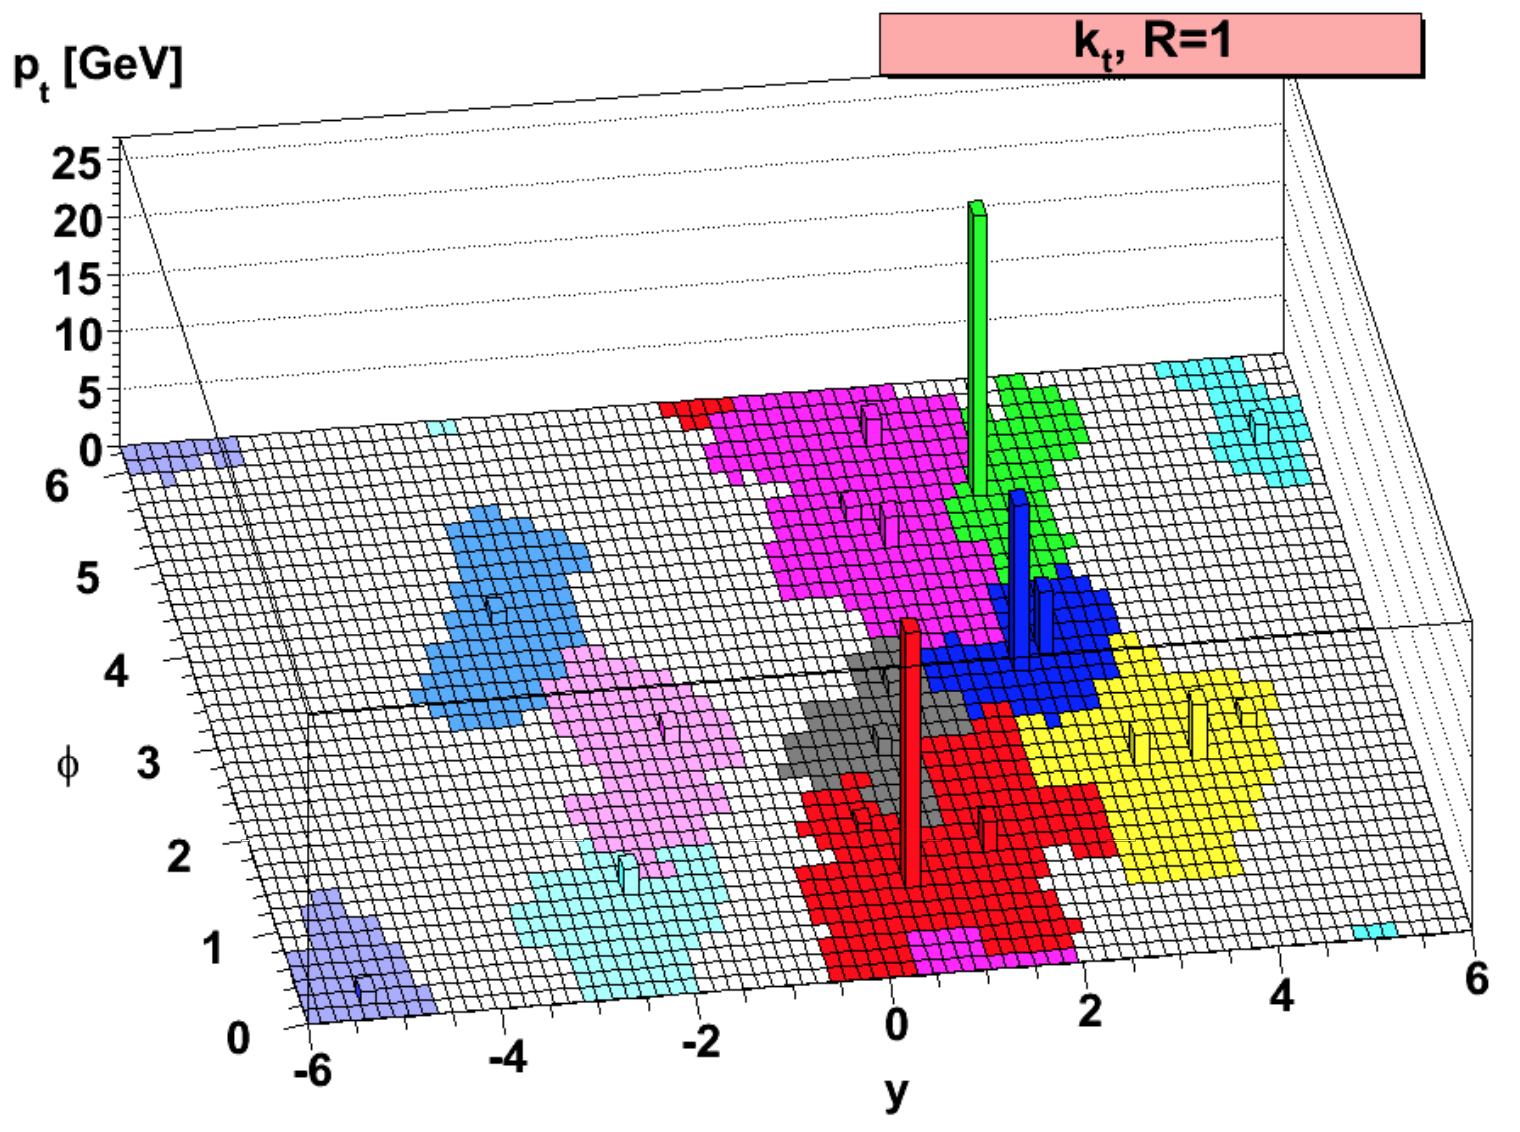
\includegraphics[width=0.32\linewidth]{figures/objects/kt}}
  \subcaptionbox{Cambridge-Aachen \label{sec:objects:Cam_Aachen}}{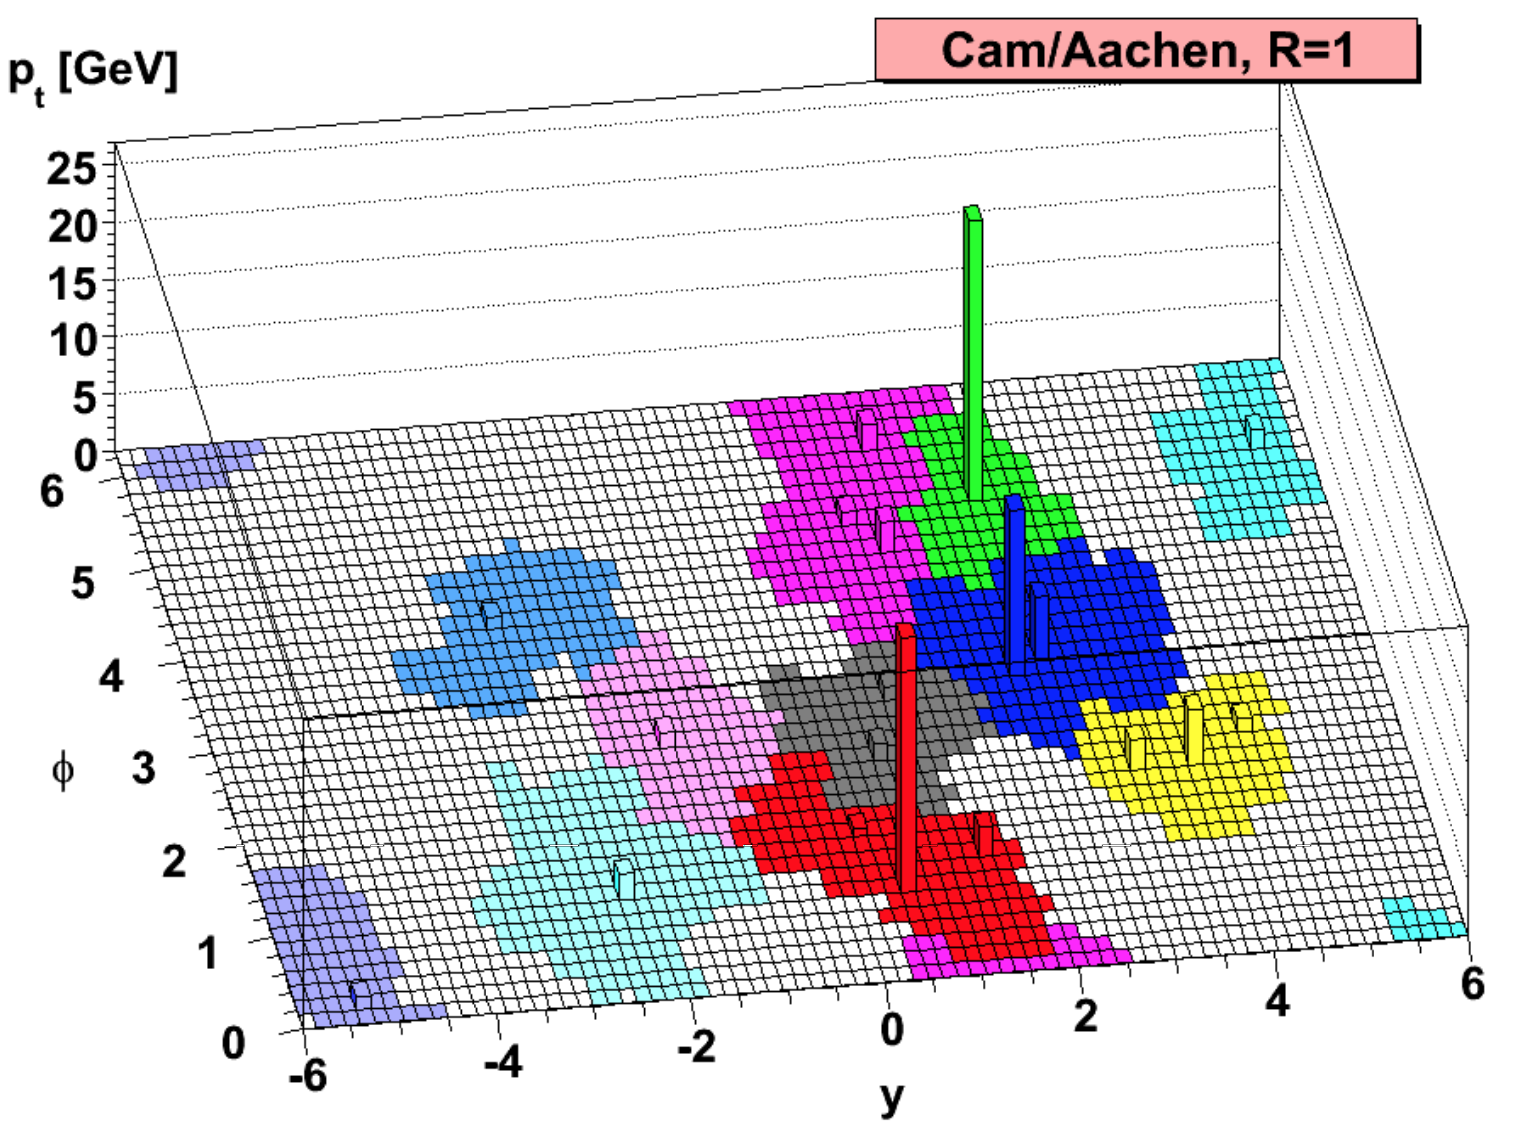
\includegraphics[width=0.32\linewidth]{figures/objects/Cam_Aachen}}
  \subcaptionbox{anti-$k_{t}$ \label{sec:objects:anti_kt}}{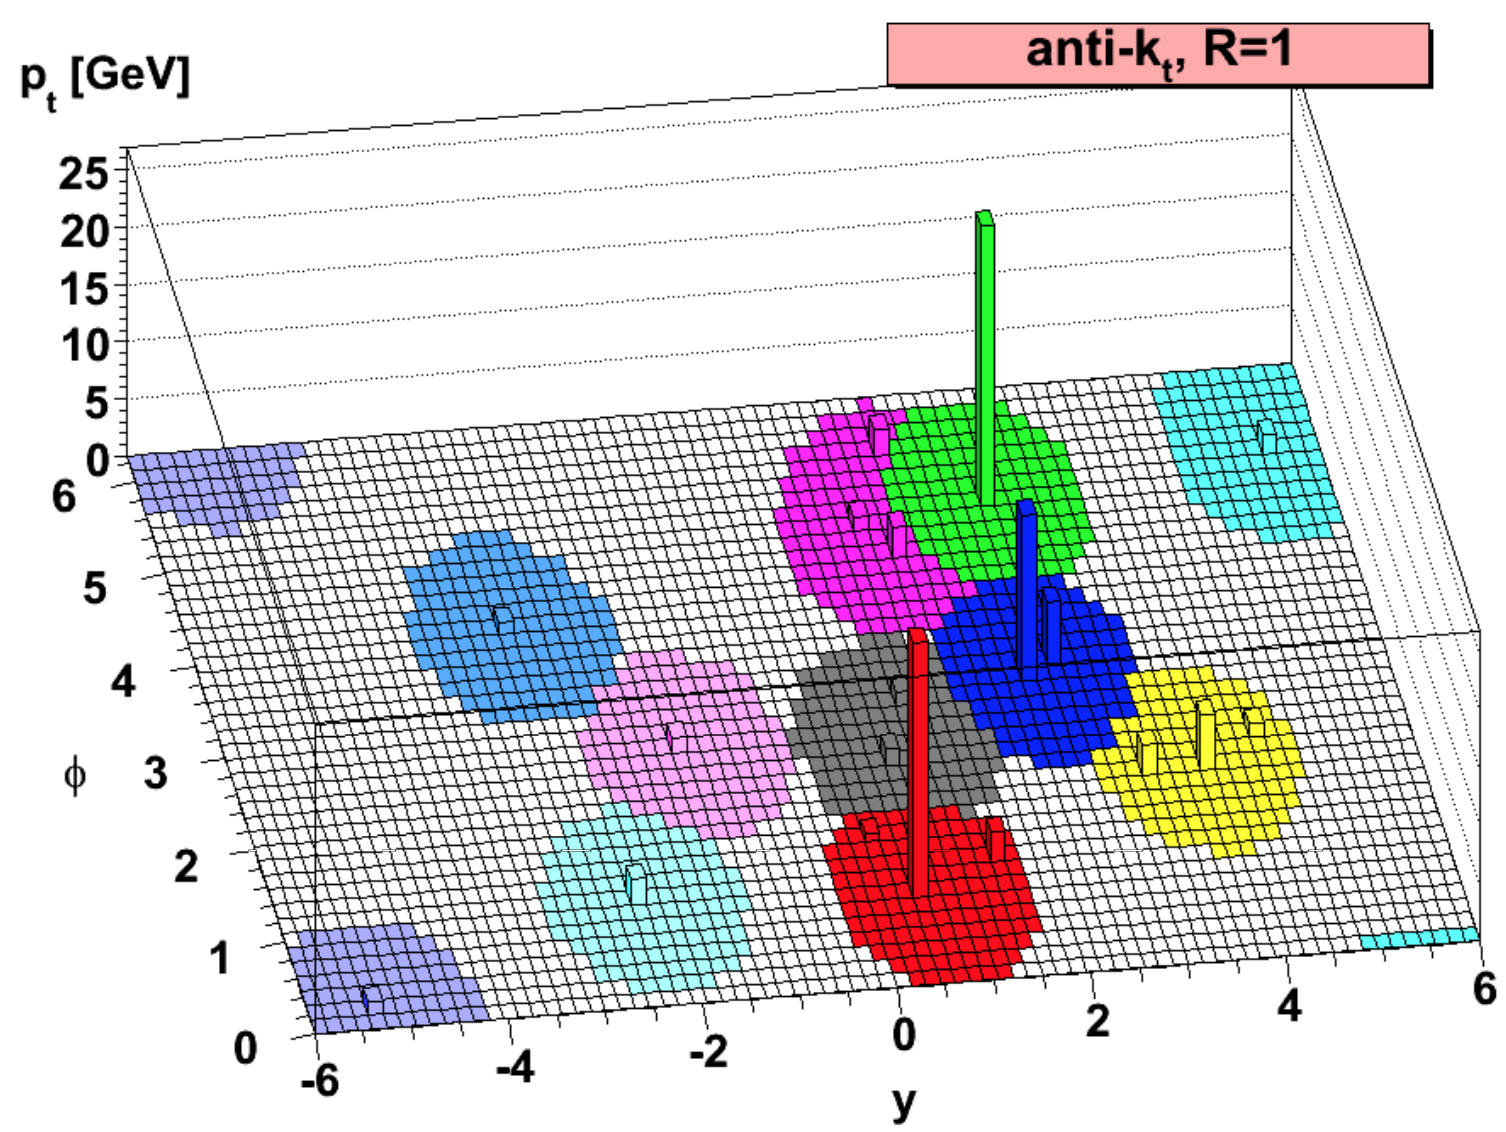
\includegraphics[width=0.32\linewidth]{figures/objects/anti_kt}}

  \caption{\cite{Cacciari:2008gp} Example clustering of a parton-level MC simulation event showing clustered jet shapes for $R=1.0$ and (a) $P=1$, (b) $P=0$, and (c) $P=-1$.}
  \label{simulated_background_shapes}
\end{figure}

\subsection{Large-$R$ Jets} \label{sec:objects:fatjet}
This thesis focuses on the boosted decay products of the Higgs boson as it
decays to $b\bar{b}$.  As discussed in \Cref{sec:higgs:boosted} the resulting
decay products are highly collimated and thus can be reconstructed using a
single large radius "large-$R$" jet where we used the typical choice of $R=1.0$
\cite{Aaboud:2018kfi,Aaboud:2017hdf}.  These large-$R$ jets are reconstructed
from topological calorimeter clusters using the anti-$k_{t}$ algorithm with a
radius parameter of $R = 1.0$ resulting in jets similar to
\Cref{sec:object:large_R_example}. After clustering we trimmed
\cite{Krohn:2009th} the large-$R$ jets to improve mass resolution and reduce
dependence on pile-up. Trimming is done by first reclustering the constituents
using the $k_{t}$ algorithm with $R=0.2$ into subjets.  Then any subjet with
$p_{T}$ less than $5\%$ of the parent large-$R$ jet's energy is removed.

\begin{figure}[!htbp]
  \centering
  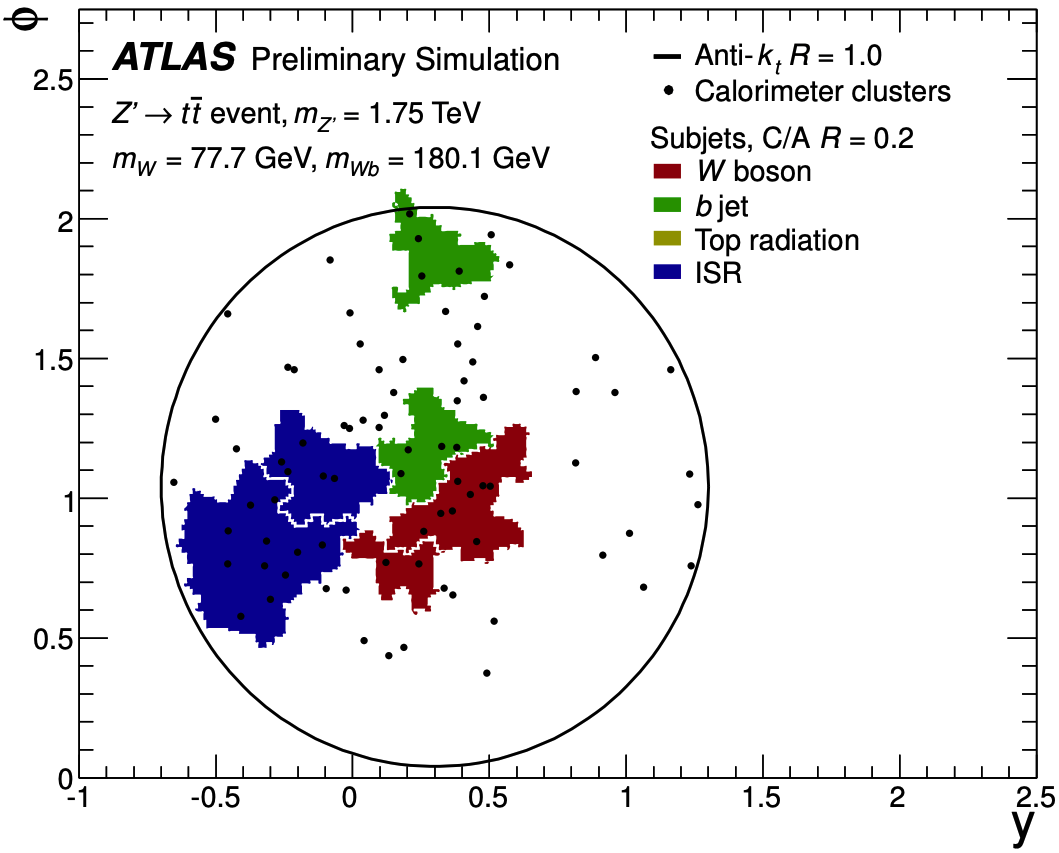
\includegraphics[width=0.7\linewidth]{figures/objects/large_R_example}
  \caption{\cite{ATLAS-CONF-2014-003} Simulation of calorimeter clusters for decay of a boosted $Z' \rightarrow t\bar{t}$ clustered in a large-$R$ jet.}
  \label{sec:object:large_R_example}
\end{figure}

\subsection{Variable Radius Track Jets} \label {sec:objects:vrjets}

After capturing the decay of the Higgs in a large-$R$ jet we must identify the
two sub-jets that represent the $b$ and $\bar{b}$ children of the Higgs. In
this thesis we chose to use the Variable Radius (VR) jet
\cite{Krohn:2009zg,ATL-PHYS-PUB-2017-010} where the clustering is accomplished
with a radius parameter $R$ which decreases as a function of the contained jet
$p_{T}$ as shown below

\[ R_{\text{eff}}(p_{T}) = \frac{\rho}{p_{T}}. \]

The constant $\rho$ determines how quickly the effective size of the VR jet
decreases with respect to the transverse momentum contained inside the jet.  In
this deifinition the choice of $\rho$ should be proportional to the mass of the
resonance $m_{\text{res}}$ you are attempting to reconstruct and should
correctly reproduce the size of jets as long as $\rho \lesssim 2p_{T}$.
Finally we choose physically motivated lower and upper bounds, $R_{\text{min}}$ and
$R_{\text{max}}$, on the size of the jet

\[
 R_{\text{eff}} \left(p_{T}\right)= \text{max}\left[\text{min}\left(\frac{\rho}{p_{T}},R_{\text{max}}\right),R_{\text{min}}\right]\,.
\]

In this thesis the variable radius track jet parameters were chosen to be $\rho
= 30\GeV$, $R_{\text{min}}=0.02$, and $R_{\text{max}}=0.4$, in order to
maximize the truth subjet double $b$-tagging efficiency for a Boosted Higgs
boson \cite{ATL-PHYS-PUB-2017-010} as seen in \Cref{vr_parameters}.  In
\Cref{sec:objects:average_deltaR} we see that the VR Track Jets properly
describe the truth $\delta R$ distribution for $b$-hadrons while the $R=0.2$
fixed track jets deviate for higher Higgs jet $p_{T}$.  Furthermore, in
\Cref{sec:objects:leading_vr} and \Cref{sec:objects:subleading_vr} we can see
that the VR track jets do a good or even better job of describing the $H
\rightarrow b\bar{b}$ topology than the $R=0.2$ fixed radius track jets.  This
ability to give a flat efficiency accross the entire Higgs $p_{T}$ spectrum
while accurately describing the topology makes these VR track jets the perfect
choice for this analysis.

\begin{figure}[!htbp]
  \centering
  \subcaptionbox{Study of $\rho$ VR track jet parameter with $R_{\text{min}} = 0.02$ and $R_{\text{max}} = 0.4$}{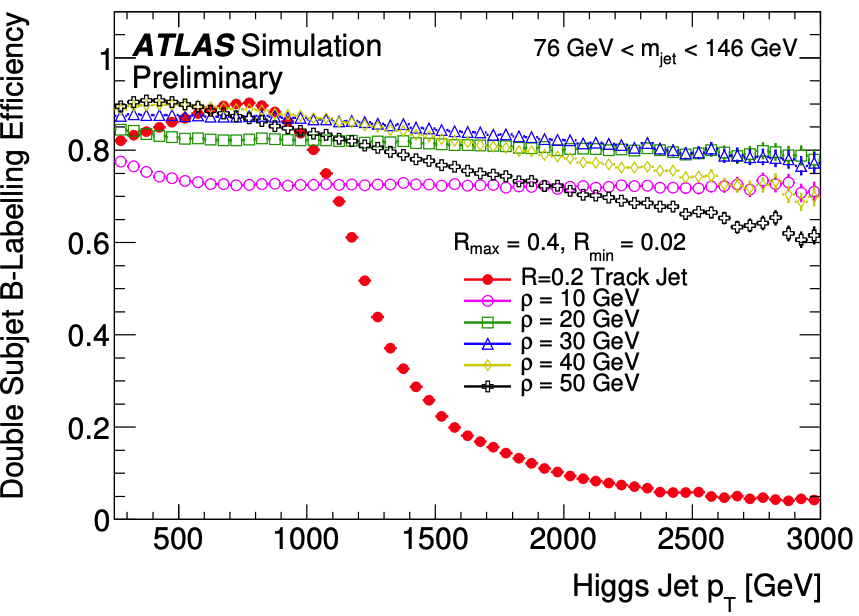
\includegraphics[width=0.48\linewidth]{figures/objects/rho}} \hfill
  \subcaptionbox{Study of $R_{\text{min}}$ VR track jet parameter with $\rho = 30\GeV$ and $R_{\text{max}} = 0.4$}{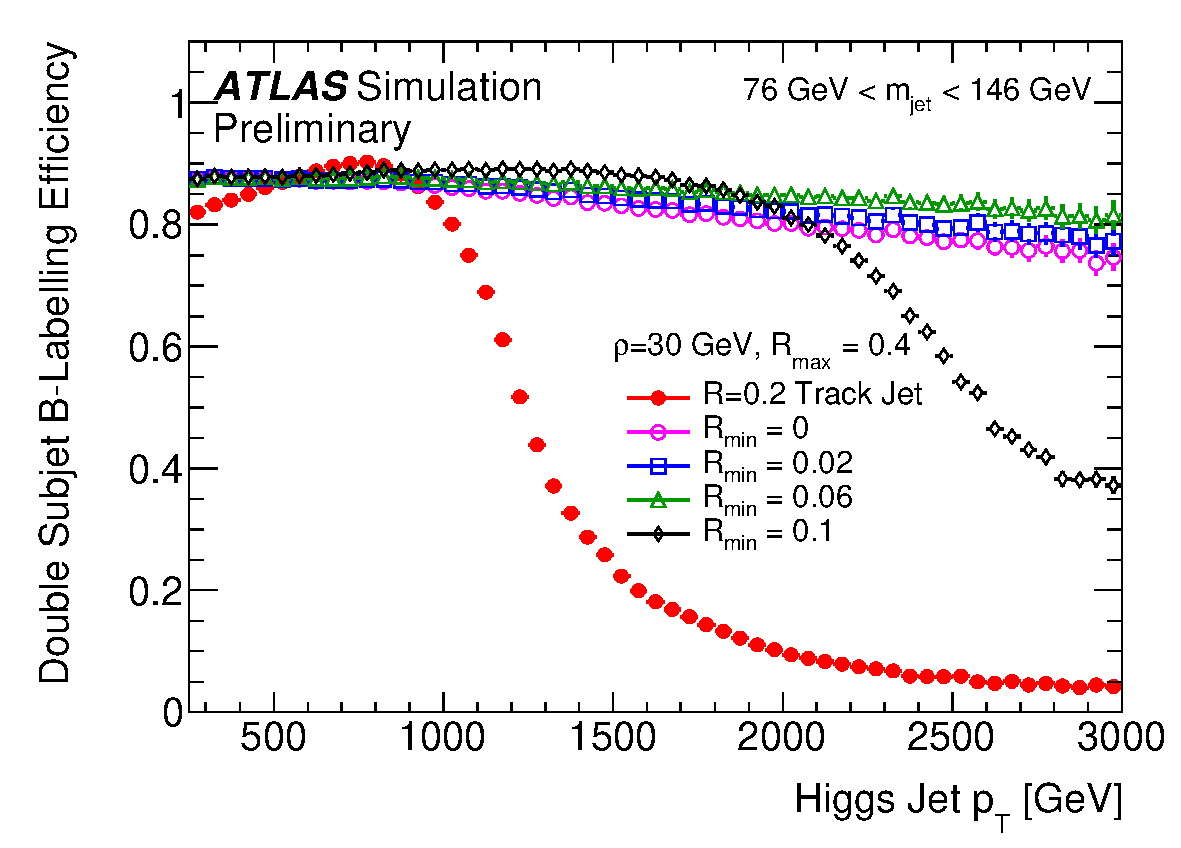
\includegraphics[width=0.48\linewidth]{figures/objects/Rmin}} \hfill
  \subcaptionbox{Study of $R_{\text{max}}$ VR track jet parameter with $\rho = 30\GeV$ and $R_{\text{min}} = 0.0.02$}{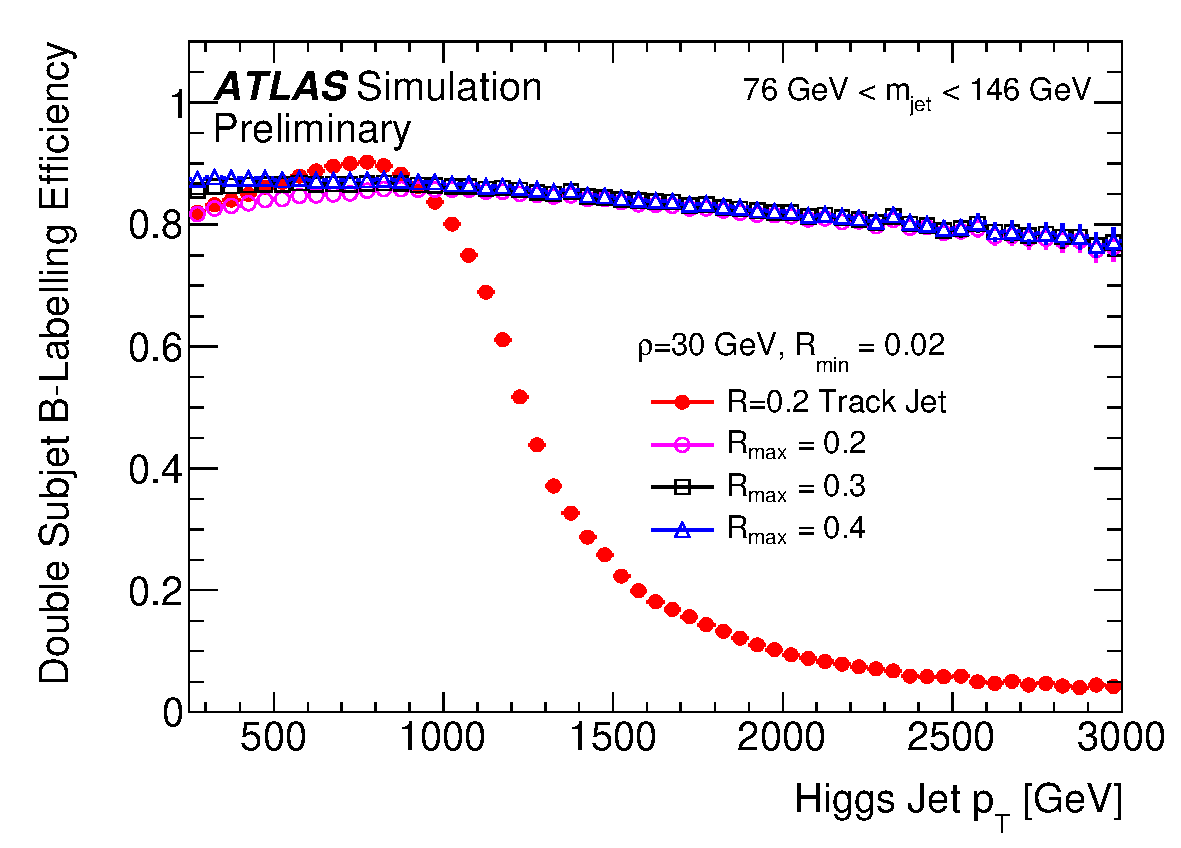
\includegraphics[width=0.48\linewidth]{figures/objects/Rmax}}

  \caption{\cite{ATL-PHYS-PUB-2017-010} Efficiency of subjet double $b$-tagging
using truth information from Higgs decay as a function of Higgs jet $p_{T}$.
The efficiency for $R=0.2$ fixed radius track jests is included for comparison.
Uncertainty bars include statistical uncertainties only.}
  \label{vr_parameters}
\end{figure}

\begin{figure}[!htbp]
  \centering
  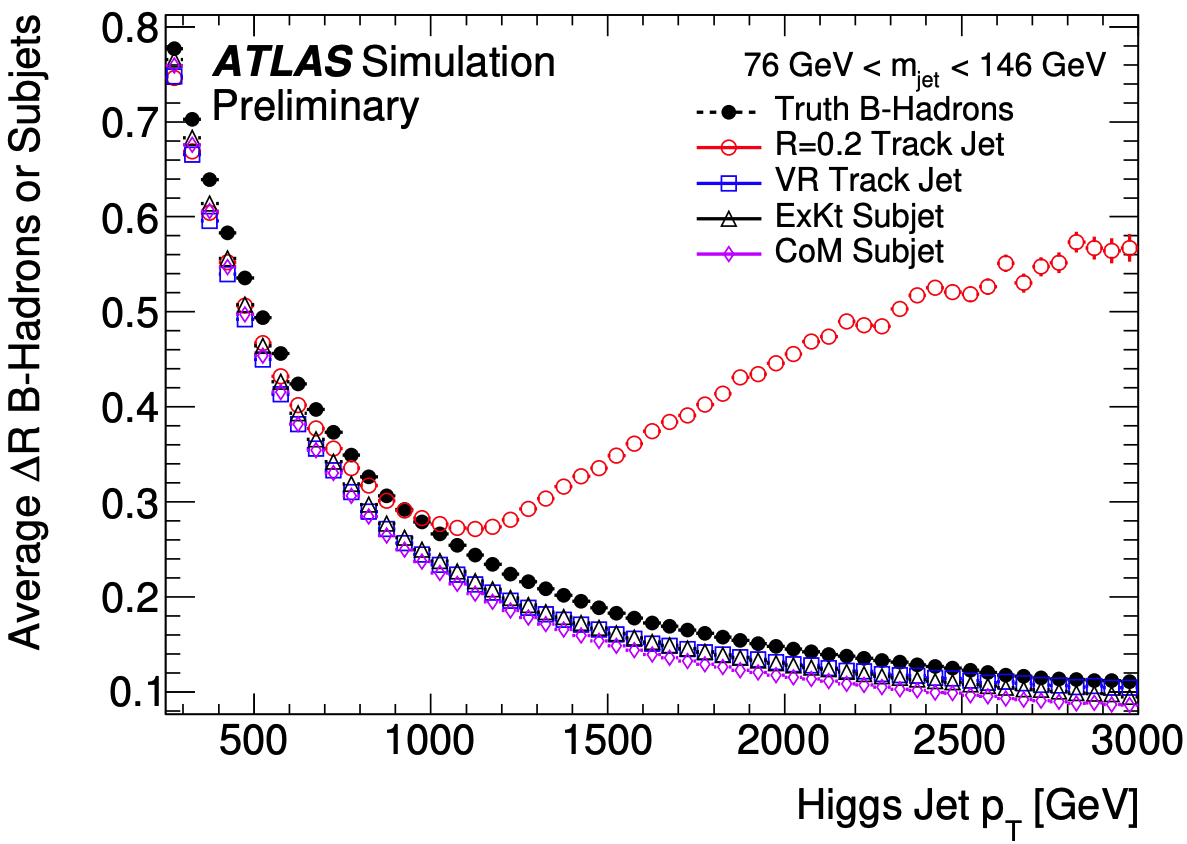
\includegraphics[width=0.98\linewidth]{figures/objects/average_deltaR}

  \caption{\cite{ATL-PHYS-PUB-2017-010} The average $\delta R$ between either
the two leading truth $b$-hadrons or the two leading subjets associated to a
Higgs jet as a function of Higgs $p_{T}$}
  \label{sec:objects:average_deltaR}
\end{figure}

\begin{figure}[!htbp]
  \centering
  \subcaptionbox{$250\GeV$ < Higgs $p_{T}$ < $400\GeV$}{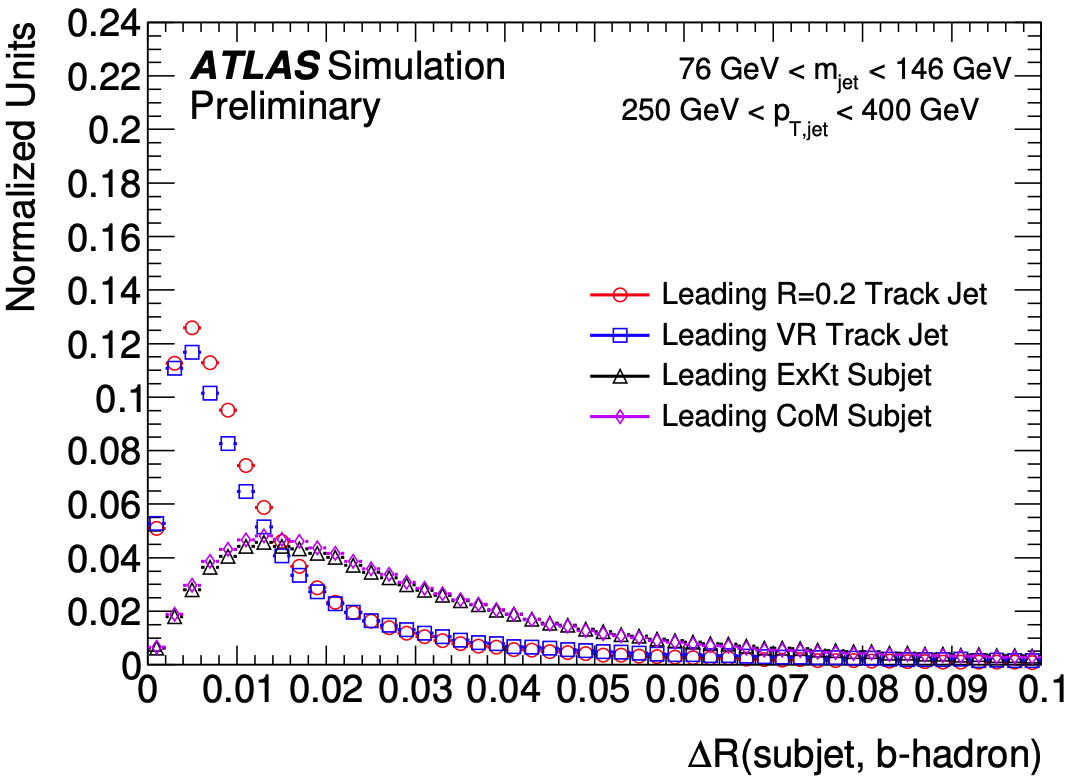
\includegraphics[width=0.48\linewidth]{figures/objects/low_leading_vr}} \hfill
  \subcaptionbox{$800\GeV$ < Higgs $p_{T}$ < $1000\GeV$}{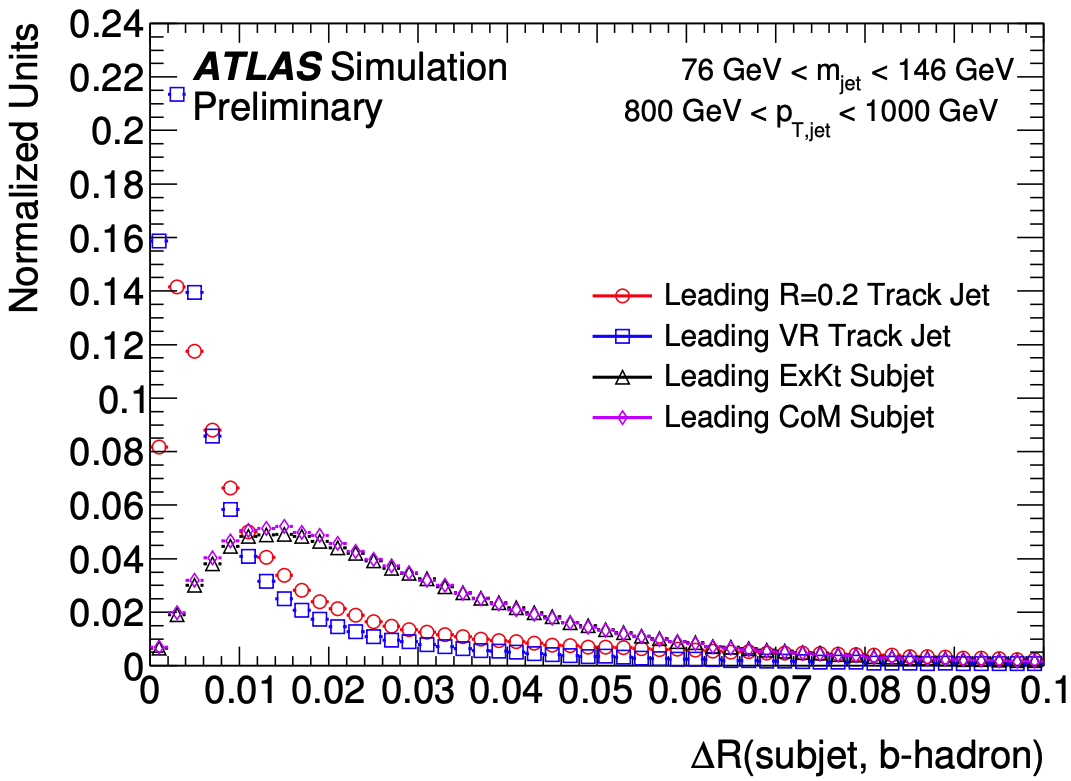
\includegraphics[width=0.48\linewidth]{figures/objects/high_leading_vr}}

  \caption{\cite{ATL-PHYS-PUB-2017-010} Distributions of $\delta R$ between a
truth matched $b$-hadron and the reconstructed leading subjet.  The
uncertainties given reflect only statistical uncertanties.  All algorithms are
normalized to an area corresponding to the fraction of signal jets which
contain a leading subjet} 
  \label{sec:objects:leading_vr}
\end{figure}

\begin{figure}[!htbp]
  \centering
  \subcaptionbox{$250\GeV$ < Higgs $p_{T}$ < $400\GeV$}{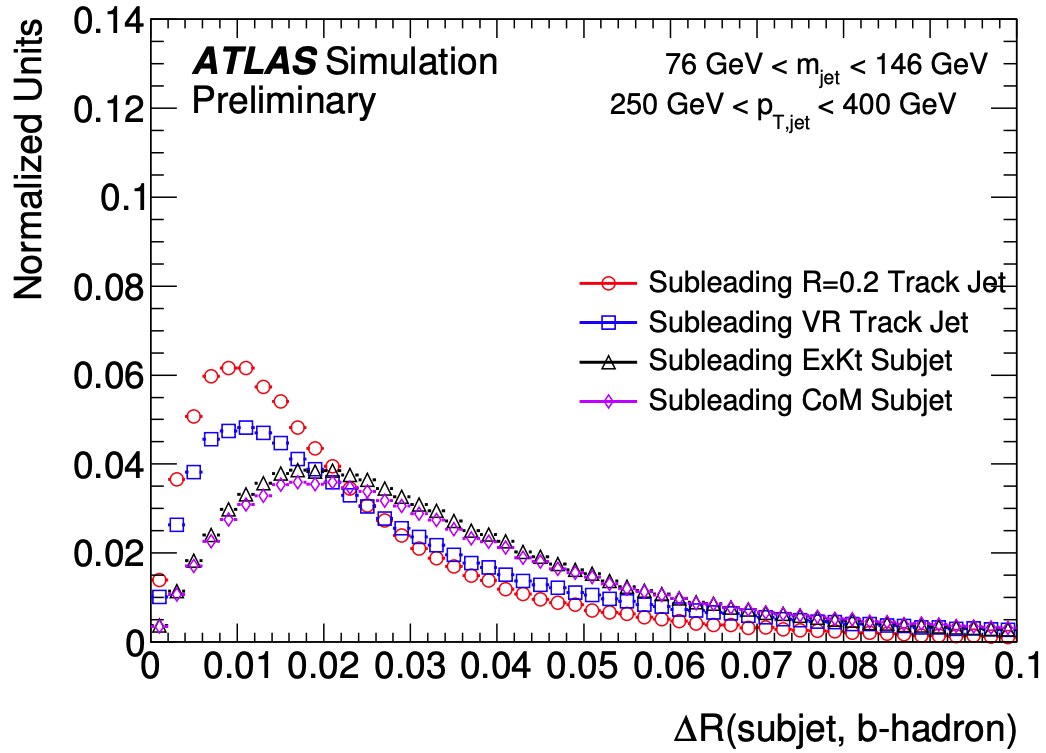
\includegraphics[width=0.48\linewidth]{figures/objects/low_subleading_vr}} \hfill
  \subcaptionbox{$800\GeV$ < Higgs $p_{T}$ < $1000\GeV$}{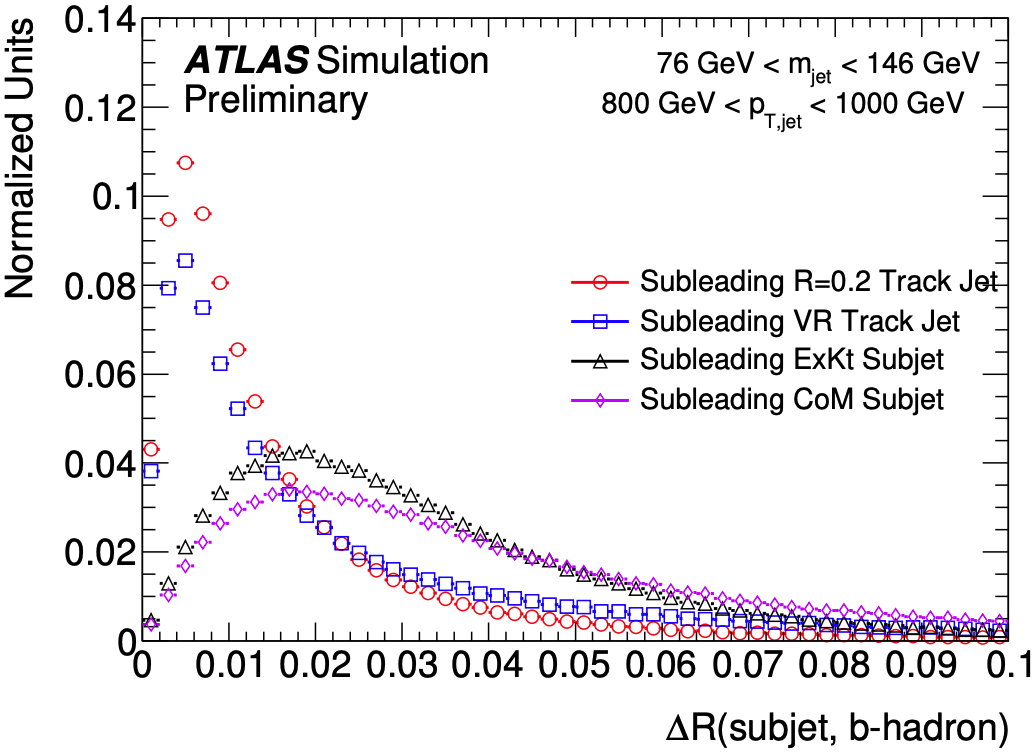
\includegraphics[width=0.48\linewidth]{figures/objects/high_subleading_vr}}

  \caption{\cite{ATL-PHYS-PUB-2017-010} Distributions of $\delta R$ between a
truth matched $b$-hadron and the reconstructed subleading subjet.  The
uncertainties given reflect only statistical uncertanties.  All algorithms are
normalized to an area corresponding to the fraction of signal jets which
contain a subleading subjet} 
  \label{sec:objects:subleading_vr}
\end{figure}



